\chapter{Tribute}


%~ \centerline{{\LARGE\sl Understanding IP Routing}}


\vskip 0.8cm

\begin{center}
{\large\uppercase{$\text{Dr. Joy A. Thomas}$}} 


\vskip -6pt

\end{center}

\vskip 2cm




\vfill




\newpage



\begin{figure}[H]
\centering
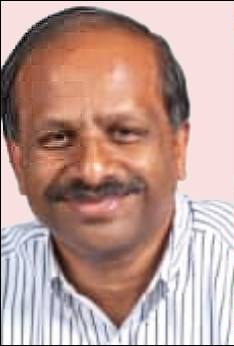
\includegraphics[scale=2]{src/Figures/fig01.jpg}
\end{figure}

\begin{center}
(Dr Joy A Thomas, a noted expert in Information Theory,\break died on Sep. 28, 2020, after a brief illness)
\end{center}

\begin{multicols}{2}
A Tribute by Arogyaswami Paulraj, Stanford University

I have known Joy’s birth family since the 1970s. Our parents were close neighbors and good friends for over three decades in Bangalore, Karnataka, India.

I did not directly witness Joy’s academic highlights at St Joseph’s Indian High School, Bangalore - I was almost a generation older and working in the Indian Navy. But I heard many stories.  His classmates recollect how he arrived atsimple and brilliant alternatesolutionsto those in the ‘Aggarwal Classes Notes’ – the gold standard prep for IIT JEE preparations in that era. Joy’s All India First Rank in IIT JEE, while still in the $11^{\rm th}$ class did not come as a surprise. He joined IIT Madras for a B.Tech. program andeasily became a legend there too. He got a perfect score in GRE and moved to Stanford University in 1984 for his Ph.D. I was then, a visiting researcher at the university, on assignment from the Indian Navy.I was happy to welcome Joy to Stanford, this brilliant boy who grew up 100 feet down the street from my parent’s house in Bangalore.

Joy chose Prof. Tom Cover, a legend in Information Theory,as his Ph.D.advisor. Some years later, Joy joined Prof. Cover, who had waited for decades for a partner with Joy’s level of genius, as a collaborator on a definitive textbook on Information Theory, an important, though abstract, subject.

Their book, “Elements of Information Theory” is regarded by many as the benchmark text on modern information theory, and a masterpiecefor clarity of concepts and the simplicity of exposition. Now, in the second edition, it remains the most popular and admired textbook on this subject around the world. There is no good academic bookstore in the world without Joy’s book. And 10,000s of Ph.D. students have learned Information Theory from his book.

After Stanford (1990), Joy joined IBM Research and later did two successful startups in the Silicon Valley – Stratify (1999) and InsightsOne (2011), acquired by apigee in 2014, which in turn was acquired by Google in 2016. He continued making seminal contributions to Predictive Analytics, working at Google, till his passing.

Joy was perhaps the most brilliant gift from India to the US in engineering sciences in recent decades. His loss is mourned by all the giants in Information Theory around the globe, from Stanford, MIT, Princeton, Berkeley, and ETH Zurich to mention a few. He will also be greatly missed in the Information Theory research community.

As a human being, Joy was gifted with wonderful qualities. Joy was a gracious and generous person. A loving father who doted on his two children Joshua and Leah, a devoted husband to his wife Priya, and to the rest of us,  a caring friend who gave us strength in time of trouble, wisdom in time of uncertainty, and sharing in time of happiness. 

Joy indeed had every gift, except the gift of long years.We all loved and admired Joy and the void left in our lives by his sudden loss can never be filled.

May his soul rest in peace.


\end{multicols}


